\chapter{The Expanding Universe}
\label{ch:universe}

\newcommand{\SixteenAge}{13.79}
\newcommand{\SixteenHubbleTime}{14.51}
\newcommand{\SixteenAgeMatterOnly}{9.67}
\newcommand{\SixteenZeqMR}{3461}
\newcommand{\SixteenZeqML}{0.30}
\newcommand{\SixteenZacc}{0.63}
\newcommand{\SixteenQzero}{-0.53}
\newcommand{\SixteenDcomovingOne}{3401}
\newcommand{\SixteenDlumOne}{6802}
\newcommand{\SixteenOmegaL}{0.685}
\newcommand{\SixteenTeqMRyr}{4.96\times10^{4}}

\newcommand{\SixteenZhalf}{1370}
\newcommand{\SixteenThalf}{3736}
\newcommand{\SixteenBoverkT}{42.3}
\newcommand{\SixteenTionise}{1.58\times10^{5}}
\newcommand{\SixteenXatThousand}{0.0037}


Distant galaxies are moving away from us, and the farther they are, the faster they go. Run the film backwards and everything was once closer, denser and hotter. The whole history of the universe on the largest scales follows from the same principles that built a star. Energy conservation for a shell of matter and the gravity of a sphere (P1, P2) give the expansion. Counting states (P3) gives the light left over from the hot beginning. Balance of rates against the rate of expansion (P4, P6) decides when atoms formed and how much helium was made. Gravity working against expansion decides how galaxies grew from tiny ripples.

General relativity, which the reader knows, gives the same equations for a uniform universe. The Newtonian route is used here because it shows where each term comes from with the least machinery.

% ==============================================================================
\section{Hubble's Law and the Scale Factor}
\label{un:sec:hubble}

Radial velocities from the Doppler shift were derived in Chapter~\ref{ch:astrometry} (Eq.~\eqref{eq:doppler_classical}).

Measured for distant galaxies, these velocities are almost all away from us. A single velocity for each galaxy says nothing about what the whole universe is doing.

Think of raisins in a rising loaf of bread. As the dough swells, every raisin moves away from every other raisin. A raisin twice as far away moves away twice as fast, and every raisin sees the same pattern, so none of them is the centre.

The universe expands like the dough. All distances between galaxies grow by the same factor at the same time. A uniform stretching makes velocity proportional to distance, which is Hubble's law, and it stretches light too, which is the cosmological redshift.

In numbers, today's expansion rate is $H_0=67.4\,\mathrm{km\,s^{-1}\,Mpc^{-1}}$. A galaxy $100\,\mathrm{Mpc}$ away recedes at $6740\,\mathrm{km\,s^{-1}}$. The time $1/H_0$ is $\SixteenHubbleTime$ billion years, the age the universe would have if it had always expanded at today's speed.

The picture is a grid drawn on a balloon. Inflating the balloon carries every grid point away from every other, while each point keeps its place on the grid.

The same uniform stretching appears in the dough, in an expanding gas and in any self-similar flow. It gives Hubble's law and the redshift in terms of one function of time, the scale factor.

\paragraph{The scale factor.} Give every galaxy fixed coordinates $\vec x$ on the stretching grid, its \textbf{comoving} position. The true distance between two galaxies is then $a(t)$ times their comoving separation, where $a(t)$ is the \textbf{scale factor}, set to $1$ today. A uniform universe has only this one function of time.

\paragraph{Hubble's law.} For a galaxy at true distance $d=a\,x$,
\begin{align}
	\dv{d}{t}
	&\eqby{1} \dv{a}{t}\,x \nonumber\\
	&\eqby{2} \frac{\dot a}{a}\,d .
\end{align}
\begin{explain}
	\item The comoving separation $x$ does not change.
	\item $x=d/a$.
\end{explain}
\begin{equation}
	\boxed{v=H\,d,\qquad H(t)\equiv\frac{\dot a}{a}.}
	\label{un:eq:hubble}
\end{equation}
The velocity is proportional to the distance, with the same $H$ for every galaxy. Every observer finds the same law, so it picks out no centre.

\paragraph{Redshift as stretching.} Light travels on the grid at $c$ in true distance, so in comoving distance it covers $c\,dt/a(t)$ in a time $dt$. Two crests leave a galaxy a time $\Delta t_{\rm e}$ apart, at scale factor $a_{\rm e}$, and arrive a time $\Delta t_0$ apart today. Both crests cover the same comoving distance, so
\begin{align}
	\int_{t_{\rm e}}^{t_0}\frac{c\,dt}{a}
	&= \int_{t_{\rm e}+\Delta t_{\rm e}}^{t_0+\Delta t_0}\frac{c\,dt}{a} \nonumber\\
	\implies\quad \frac{\Delta t_{\rm e}}{a_{\rm e}}
	&\eqby{1} \frac{\Delta t_0}{a_0} .
\end{align}
\begin{explain}
	\item Subtract the common part of the two integrals. What is left are two short pieces, of length $\Delta t_{\rm e}$ at the start and $\Delta t_0$ at the end, during which $a$ hardly changes.
\end{explain}
The wavelength is $c$ times the time between crests, so it grows in proportion to the scale factor,
\begin{equation}
	\boxed{1+z\equiv\frac{\lambda_{\rm obs}}{\lambda_{\rm emit}}=\frac{a_0}{a_{\rm e}}=\frac{1}{a_{\rm e}}.}
	\label{un:eq:redshift}
\end{equation}
The redshift measures how much the universe has grown since the light left, not a velocity. For small distances it reduces to the Doppler form $z\approx v/c$ with $v=Hd$.

% ==============================================================================
\section{The Friedmann Equations}
\label{un:sec:friedmann}

Hubble's law describes the expansion today. Chapter~\ref{ch:twobody} and Section~\ref{sg:sec:freefall} followed a single body or a single shell moving under gravity.

The expansion is not free. Every galaxy pulls on every other, so gravity should slow the expansion, and how $a(t)$ changes depends on what the universe contains.

Throw a ball straight up. If it goes fast enough it escapes the Earth, and if not it falls back. The answer depends only on its energy, kinetic against the depth of the gravitational well.

Take any sphere in a uniform universe. By P2, a shell on its surface feels only the mass inside, so it moves exactly like the thrown ball, with energy conserved (P1). Writing that energy in terms of the scale factor gives the Friedmann equation, the equation of motion of the whole universe.

The ball in numbers. The escape speed from the Earth is $11.2\,\mathrm{km\,s^{-1}}$. For the universe the same balance defines a critical density, $3H_0^2/(8\pi G)=8.5\times10^{-27}\,\mathrm{kg\,m^{-3}}$, about five hydrogen atoms per cubic metre.

The picture is a sphere carved out of the universe, its surface shell flying outward and slowing under the pull of what it contains.

The same equation comes out of general relativity for any uniform universe, with the energy constant reinterpreted as the curvature of space. It gives the expansion rate, how each kind of content dilutes, whether the expansion speeds up, and the age.

\paragraph{The energy of a shell.} Take a sphere of comoving radius $x$, true radius $r=a\,x$ and density $\rho$. The mass inside, $M=\tfrac43\pi\rho a^3x^3$, stays constant as the shell moves with the expansion. Energy conservation per unit mass of the shell (P1, with P2 for the gravity) reads
\begin{align}
	\frac12\dot r^2-\frac{GM}{r}
	&= \text{constant} \nonumber\\
	\implies\quad \frac12\dot a^2x^2-\frac43\pi G\rho\,a^2x^2
	&\eqby{1} \text{constant} \nonumber\\
	\implies\quad \left(\frac{\dot a}{a}\right)^2
	&\eqby{2} \frac{8\pi G}{3}\,\rho-\frac{kc^2}{a^2} .
\end{align}
\begin{explain}
	\item $r=ax$ and $M=\tfrac43\pi\rho a^3x^3$.
	\item Divide by $\tfrac12a^2x^2$, and write the constant as $-kc^2/(2x^2)$, which defines $k$. It is the same for every shell because the universe is uniform.
\end{explain}
\begin{equation}
	\boxed{H^2=\frac{8\pi G}{3}\,\rho-\frac{kc^2}{a^2}.}
	\label{un:eq:friedmann}
\end{equation}
This is the \textbf{Friedmann equation}. General relativity gives exactly this form, with $\rho$ the total energy density divided by $c^2$ and $k$ the curvature of space. The universe is observed to be flat to good accuracy, so from here on $k=0$, and then the density is fixed by the expansion rate,
\begin{equation}
	\rho_{\rm crit}=\frac{3H^2}{8\pi G},\qquad \Omega_i\equiv\frac{\rho_{i,0}}{\rho_{\rm crit,0}} .
	\label{un:eq:critical}
\end{equation}
Each content $i$ (matter, radiation, the cosmological constant) is described by its share $\Omega_i$ of the critical density today.

\paragraph{How each content dilutes.} The Friedmann equation needs $\rho(a)$. Take a comoving volume $V\propto a^3$. Its energy $\rho c^2V$ changes only by the work done by its pressure as it expands (P1, the first law with no heat flowing in a uniform universe),
\begin{align}
	d(\rho c^2a^3)
	&= -P\,d(a^3) \nonumber\\
	\implies\quad \dot\rho+3\frac{\dot a}{a}\left(\rho+\frac{P}{c^2}\right)
	&\eqby{1} 0 .
	\label{un:eq:fluid}
\end{align}
\begin{explain}
	\item Divide by $c^2a^3\,dt$ and use $d(a^3)=3a^2\,da$.
\end{explain}
With $P=w\rho c^2$ for a fixed $w$, this integrates to $\rho\propto a^{-3(1+w)}$. Three cases matter.
\begin{itemize}
	\item Matter, $w=0$ (pressure negligible), $\rho\propto a^{-3}$. The particles are only spread over a larger volume.
	\item Radiation, $w=\tfrac13$ (Eq.~\eqref{pr:eq:P_u}), $\rho\propto a^{-4}$. Each photon is also redshifted, losing one more power of $a$.
	\item A cosmological constant, $w=-1$, $\rho=$ constant. Its energy density does not dilute at all.
\end{itemize}
So for a flat universe
\begin{equation}
	\boxed{H^2=H_0^2\left(\frac{\Omega_m}{a^3}+\frac{\Omega_r}{a^4}+\Omega_\Lambda\right),\qquad \Omega_m+\Omega_r+\Omega_\Lambda=1.}
	\label{un:eq:friedmann_omegas}
\end{equation}
Radiation rules when $a$ is small, then matter, then the cosmological constant. Matter and radiation were equal at $1+z=\Omega_m/\Omega_r$, $z\approx\SixteenZeqMR$, when the universe was about $\SixteenTeqMRyr$ years old.

\paragraph{Does the expansion slow down?} Differentiate Eq.~\eqref{un:eq:friedmann} (with $k=0$) in time and use the fluid equation,
\begin{align}
	2\frac{\dot a}{a}\left(\frac{\ddot a}{a}-\frac{\dot a^2}{a^2}\right)
	&\eqby{1} \frac{8\pi G}{3}\,\dot\rho \nonumber\\
	&\eqby{2} -8\pi G\,\frac{\dot a}{a}\left(\rho+\frac{P}{c^2}\right) \nonumber\\
	\implies\quad \frac{\ddot a}{a}
	&\eqby{3} -\frac{4\pi G}{3}\left(\rho+\frac{3P}{c^2}\right).
\end{align}
\begin{explain}
	\item $\dv*{}{t}(\dot a/a)=\ddot a/a-\dot a^2/a^2$.
	\item The fluid equation \eqref{un:eq:fluid}.
	\item Divide by $2\dot a/a$ and replace $\dot a^2/a^2$ by $(8\pi G/3)\rho$.
\end{explain}
\begin{equation}
	\boxed{\frac{\ddot a}{a}=-\frac{4\pi G}{3}\left(\rho+\frac{3P}{c^2}\right).}
	\label{un:eq:acceleration}
\end{equation}
Ordinary matter and radiation slow the expansion. Pressure adds to the pull, as it did in the TOV equation (Section~\ref{cs:sec:relativistic}). A content with $w<-\tfrac13$ makes $\rho+3P/c^2<0$ and speeds the expansion up. A cosmological constant, $w=-1$, does.

\paragraph{Single-content universes.} With one content at a time, Eq.~\eqref{un:eq:friedmann_omegas} integrates directly. For matter only, $\dot a=H_0a^{-1/2}$, so $a^{1/2}da=H_0\,dt$ and
\begin{equation}
	a=\left(\tfrac32H_0t\right)^{2/3},\qquad t_0=\frac{2}{3H_0}=\SixteenAgeMatterOnly\ \text{Gyr}.
\end{equation}
For radiation only, $a=(2H_0t)^{1/2}$ and $t_0=1/(2H_0)$. For a cosmological constant only, $a=e^{H_0(t-t_0)}$, with no beginning at all. Expansion that is always slowing has an age shorter than $1/H_0$.

\paragraph{Our universe.} For the Planck values $H_0=67.4\,\mathrm{km\,s^{-1}\,Mpc^{-1}}$, $\Omega_m=0.315$, $\Omega_r=9.1\times10^{-5}$ and $\Omega_\Lambda=\SixteenOmegaL$, the age is found by integrating $dt=da/(aH)$ from $a=0$ to $1$ on the cluster,
\begin{equation}
	\boxed{t_0=\int_0^1\frac{da}{a\,H(a)}=\SixteenAge\ \text{Gyr}.}
	\label{un:eq:age}
\end{equation}
This is longer than the matter-only age, because the cosmological constant has sped up the expansion lately, and close to $1/H_0$ by coincidence. Figure~\ref{un:fig:scale_factor} compares the four histories. The oldest stars, about $13$ billion years old, fit inside this age, as they must.

\begin{figure}[htbp]
	\centering
	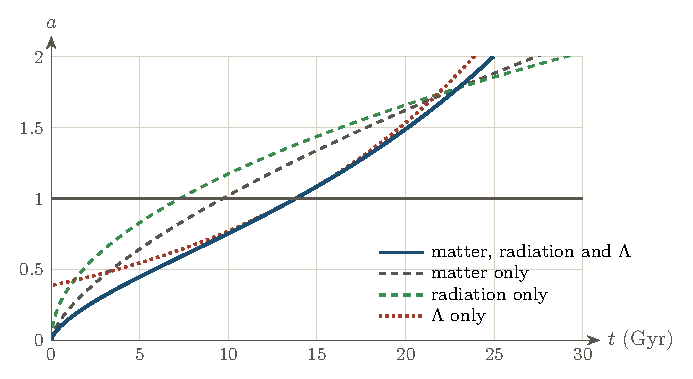
\includegraphics{fig_ch16_scale_factor.pdf}
	\caption{The scale factor against time for a flat universe with matter, radiation and a cosmological constant (Planck 2018 values), and for universes with only matter, only radiation or only a cosmological constant, each with the same $H_0$ when $a=1$.}
	\label{un:fig:scale_factor}
\end{figure}

% ==============================================================================
\section{The Microwave Background and Recombination}
\label{un:sec:cmb}

Light in thermal equilibrium has the Planck spectrum (Eq.~\eqref{pr:eq:planck}), and the universe was once dense and hot.

Today the universe is cold, thin and transparent. If its early light is still around, it has been stretched by expansion for billions of years, and it is not obvious that it should still look thermal, or when it last met matter.

Think of a guitar string in a box that slowly grows. Each note the string can play gets lower as the box grows, but the set of notes keeps the same pattern, only shifted. Light in an expanding universe is like that. Every mode is stretched by the same factor.

The early universe was full of light in equilibrium with matter. As it expanded, every photon's wavelength grew with $a$, the number of photons in each mode stayed the same (P1), and the Planck spectrum stayed a Planck spectrum at a temperature falling as $1/a$ (P3). When the universe cooled enough for electrons to join protons, the light was set free. The temperature at which that happened is set by counting states (P3), detailed balance (P4) and one ratio, the enormous number of photons per atom (P6).

In numbers, the light is seen today at $2.7255\,\mathrm{K}$, $411$ photons per cubic centimetre. It was released at about $3000\,\mathrm K$, far below the $1.58\times10^5\,\mathrm K$ at which a typical photon carries hydrogen's ionisation energy.

The picture is a fog that suddenly clears. Before, light scatters off free electrons at every step. After, the electrons are locked in atoms and the light flies straight, carrying a snapshot of the moment the fog lifted.

The same counting gives the ionisation of gas in stellar atmospheres and nebulae, and the same photon excess sets when the first nuclei formed (Section~\ref{un:sec:bbn}). It gives the temperature law, the photon density and the Saha equation.

\paragraph{A blackbody stays a blackbody.} Between interactions, each photon's momentum falls as $1/a$, by Eq.~\eqref{un:eq:redshift}. The number of photons in a given set of modes does not change, and the modes themselves are carried along with $p\propto1/a$. The occupation of a mode, $f=1/(e^{pc/k_BT}-1)$ in equilibrium (Section~\ref{pr:sec:p3}), is therefore unchanged if $pc/k_BT$ stays the same for each mode,
\begin{equation}
	\boxed{T\propto\frac1a,\qquad T=T_0(1+z).}
	\label{un:eq:T_scaling}
\end{equation}
The spectrum keeps the Planck form exactly, at a temperature falling as the universe grows. It is measured today at $T_0=2.7255\,\mathrm K$, the most perfect blackbody known. Hot gas in galaxy clusters scatters a small part of it to higher energies, so at low frequencies clusters appear as faint cool spots on the microwave sky, the Sunyaev–Zel'dovich effect of Eq.~\eqref{fp:eq:sz}.

\paragraph{How many photons.} With Eq.~\eqref{pr:eq:dn}, two polarisations and $x=pc/k_BT$,
\begin{align}
	n_\gamma
	&\eqby{1} \int_0^\infty\frac{2}{h^3}\,\frac{4\pi p^2\,dp}{e^{pc/k_BT}-1} \nonumber\\
	&\eqby{2} 8\pi\left(\frac{k_BT}{hc}\right)^3\int_0^\infty\frac{x^2\,dx}{e^x-1} \nonumber\\
	&\eqby{3} 16\pi\zeta(3)\left(\frac{k_BT}{hc}\right)^3 .
\end{align}
\begin{explain}
	\item Counting states, Eq.~\eqref{pr:eq:dn}, with the Planck occupation.
	\item The substitution $x=pc/k_BT$.
	\item $\int_0^\infty x^2dx/(e^x-1)=2\zeta(3)=2.404$, where $\zeta(3)=1.202$.
\end{explain}
At $T_0=2.7255\,\mathrm K$ this gives $n_\gamma=411\,\mathrm{cm^{-3}}$. The energy density is $a_{\rm rad}T_0^4$ (Eq.~\eqref{pr:eq:photon_gas}, with the radiation constant written $a_{\rm rad}$, since $a$ is now the scale factor), which is a share $\Omega_\gamma=5.4\times10^{-5}$ of the critical density. Neutrinos add $68\%$ more, giving the $\Omega_r=9.1\times10^{-5}$ used above. Ordinary matter, $\Omega_b=0.049$, has $\eta=n_b/n_\gamma=6.1\times10^{-10}$ baryons per photon. This tiny ratio decides the next result.

\paragraph{The Saha equation.} Hydrogen is ionised and re-formed by $\mathrm p+\mathrm e\rightleftharpoons\mathrm H+\gamma$. In equilibrium, each process is balanced by its reverse (P4), so the populations take their equilibrium ratio from counting states (P3). A bound atom in its ground state has energy $-B$, with $B=13.6\,\mathrm{eV}$. Ionising it frees an electron, which can then take any of the translational states available to it. An electron sharing space with the other free electrons has a volume $1/n_e$ to itself, and by Eq.~\eqref{pr:eq:states} the number of its momentum states up to a thermal momentum is about $(2\pi m_ek_BT/h^2)^{3/2}/n_e$ (the Maxwell distribution integrated over $d^3p/h^3$). The Boltzmann factor for the energy $B$ completes the ratio (the spin states of electron, proton and atom cancel, $2\times2/4=1$),
\begin{equation}
	\boxed{\frac{n_pn_e}{n_{\rm H}}=\left(\frac{2\pi m_ek_BT}{h^2}\right)^{3/2}e^{-B/k_BT}.}
	\label{un:eq:saha}
\end{equation}
This is the \textbf{Saha equation}. With the ionised fraction $x=n_e/n_{\rm H,tot}$ and $n_p=n_e$, it becomes
\[
\frac{x^2}{1-x}=\frac{1}{n_{\rm H,tot}}\left(\frac{2\pi m_ek_BT}{h^2}\right)^{3/2}e^{-B/k_BT},\qquad n_{\rm H,tot}=(1-Y)\,\eta\,n_\gamma ,
\]
with $Y=0.245$ the helium mass fraction (Section~\ref{un:sec:bbn}).

\paragraph{Why so cold?} The bracket grows as $T^{3/2}$, while $n_{\rm H,tot}=(1-Y)\eta n_\gamma$ grows as $T^3$, so the right side is roughly
\[
\frac{1}{\eta}\left(\frac{m_ec^2}{k_BT}\right)^{3/2}e^{-B/k_BT}\times\text{(a number of order one)}.
\]
The factor $1/\eta\approx1.6\times10^9$ is huge. Each atom that forms is surrounded by over a billion photons, and even far out on their Planck tail enough of them carry $13.6\,\mathrm{eV}$ to break it again. Hydrogen stays ionised until $e^{-B/k_BT}$ has fallen far enough to beat $10^9$ (P6). The script solves for $x$ against $z$ (Figure~\ref{un:fig:saha}). The fraction falls through one half at $z=\SixteenZhalf$, $T=\SixteenThalf\,\mathrm K$, where $B/k_BT=\SixteenBoverkT$, against the $\SixteenTionise\,\mathrm K$ at which $k_BT=B$.

\begin{figure}[htbp]
	\centering
	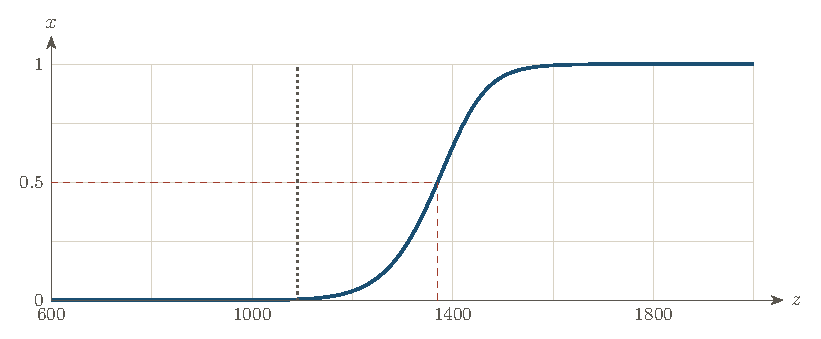
\includegraphics{fig_ch16_saha.pdf}
	\caption{The ionised fraction of hydrogen against redshift from the Saha equation. The dashed lines mark $x=\tfrac12$. The dotted line marks $z=1090$.}
	\label{un:fig:saha}
\end{figure}

Real recombination lags a little behind Saha's equilibrium. Each atom that forms in its ground state emits a photon that can ionise its neighbour, so the last stages are slowed and the light decouples at $z\approx1090$, $T\approx3000\,\mathrm K$, where the photons' mean free path grows past the size of the universe (P6, as in Section~\ref{rad:sec:transfer}). That moment, about $380\,000$ years after the start, is what the microwave background shows.

% ==============================================================================
\section{Freeze-Out and the First Three Minutes}
\label{un:sec:bbn}

Recombination happened when a reaction balance shifted as the universe cooled (Section~\ref{un:sec:cmb}).

Earlier, at temperatures of billions of kelvin, the same kind of balance governed the nuclei. One more effect then matters. A reaction can only keep its balance if it runs faster than the universe changes.

Think of a party where guests keep swapping partners. While the room is crowded, swaps are frequent and partners stay mixed. As guests leave and the room empties, encounters become rare, and at some point everyone is stuck with whoever they last danced with. The mix freezes in at the moment encounters become rarer than the room changes.

In the early universe, neutrons and protons turned into each other through weak reactions with electrons and neutrinos. While those reactions ran faster than the expansion (P4), the neutron-to-proton ratio followed its equilibrium value from the Boltzmann factor (P3). When the expansion overtook them (P6), the ratio froze, and almost all the neutrons that remained ended up in helium.

In numbers, the ratio froze at about one neutron for five protons. Some neutrons decayed before nuclei could form, leaving one for seven, which makes a quarter of the mass into helium.

The picture is two curves crossing, the reaction rate falling steeply as the universe cools and the expansion rate falling gently, with the freeze-out where they cross.

The same freeze-out decides how much dark matter is left over if it is a particle, when neutrinos stopped interacting, and the amounts of deuterium and lithium. It gives the time–temperature relation, the freeze-out ratio, the helium fraction and the deuterium delay.

\paragraph{Time and temperature.} Early on, radiation dominates and $\rho\propto a^{-4}$, so $\dot a/a\propto a^{-2}$ gives $a\propto t^{1/2}$ and $H=1/(2t)$. The Friedmann equation then ties the time to the temperature. With $\rho c^2=g\,\tfrac12a_{\rm rad}T^4$, where $g=10.75$ counts photons, electrons, positrons and three kinds of neutrino at a few MeV (fermions counting $\tfrac78$ of a boson),
\begin{align}
	\frac{1}{4t^2}
	&\eqby{1} \frac{8\pi G}{3}\,\frac{g\,a_{\rm rad}T^4}{2c^2} \nonumber\\
	\implies\quad t
	&= \left(\frac{3c^2}{16\pi G\,g\,a_{\rm rad}}\right)^{1/2}\frac{1}{T^2}
	\eqby{2} 0.74\,\mathrm s\left(\frac{1\,\mathrm{MeV}}{k_BT}\right)^2 .
\end{align}
\begin{explain}
	\item $H=1/(2t)$ in the Friedmann equation, with each species' share of the radiation energy density.
	\item Numbers for $g=10.75$.
\end{explain}
A second after the beginning the temperature was about $10^{10}\,\mathrm K$, and three minutes after it about $10^9\,\mathrm K$.

\paragraph{The freeze-out condition.} The weak reactions $\mathrm n+\nu\rightleftharpoons\mathrm p+\mathrm e$ and $\mathrm n+\mathrm e^+\rightleftharpoons\mathrm p+\bar\nu$ have a cross-section that grows as the square of the energy, so their rate per nucleon grows as $T^5$ (density $\propto T^3$, speed $c$, cross-section $\propto T^2$). The expansion rate grows only as $T^2$. The ratio of the two falls as $T^3$, and the reactions stop keeping up when
\begin{equation}
	\boxed{\Gamma\approx H.}
	\label{un:eq:freeze}
\end{equation}
With the measured strength of the weak interaction this happens at $k_BT_f\approx0.8\,\mathrm{MeV}$.

\paragraph{Neutrons and helium.} Before freeze-out the reactions in each direction balance (P4), and the Boltzmann factor of Eq.~\eqref{pr:eq:detailed_balance} gives
\[
\frac np=e^{-Q/k_BT},\qquad Q=(m_n-m_p)c^2=1.293\,\mathrm{MeV}.
\] At freeze-out this is $e^{-1.293/0.8}=0.20$. Free neutrons then decay, with a mean life of $879\,\mathrm s$. Almost every neutron left when nuclei finally form, at about $t\approx200\,\mathrm s$, ends up in helium-4, which holds two neutrons and two protons. With $n/p$ the ratio at that moment, the mass fraction in helium is
\begin{align}
	Y
	&\eqby{1} \frac{4\,(n/2)}{n+p}
	= \frac{2\,(n/p)}{1+n/p}
	\eqby{2} \frac{2\times\tfrac17}{1+\tfrac17}=0.25 .
\end{align}
\begin{explain}
	\item Each helium nucleus uses two neutrons and has four times the nucleon mass, so the helium mass is $4\times n/2$ in units of the nucleon mass, out of a total $n+p$.
	\item After freeze-out and decay, $n/p\approx\tfrac17$.
\end{explain}
The measured primordial helium fraction is $0.245$. A crude model with freeze-out at $0.8\,\mathrm{MeV}$ and nuclei forming at $180\,\mathrm s$ gives $n/p=0.16$ and $Y=0.28$. The full calculation, which follows the reaction rates through the freeze-out instead of cutting them off, gives $n/p\approx\tfrac17$ and agrees with the measurement.

\paragraph{The deuterium bottleneck.} Helium forms through deuterium, bound by only $2.22\,\mathrm{MeV}$. As with hydrogen in Section~\ref{un:sec:cmb}, a billion photons per nucleon can break every deuteron as long as enough photons on the Planck tail carry $2.22\,\mathrm{MeV}$. Deuterium survives only once $e^{-B_D/k_BT}$ has fallen below about $\eta$,
\begin{equation}
	k_BT\approx\frac{B_D}{\ln(1/\eta)}=\frac{2.22\,\mathrm{MeV}}{21.2}\approx0.1\,\mathrm{MeV},
\end{equation}
and the full Saha-type balance, which adds the slowly varying factors, lowers this to $0.07\,\mathrm{MeV}$, about $8\times10^8\,\mathrm K$. By the time-temperature relation that is about three minutes, the time the neutrons had to decay. The same photon excess that delayed recombination delayed the first nuclei. The tunnelling that makes fusion possible at these energies is that of Section~\ref{st:sec:eos}.

% ==============================================================================
\section{The Growth of Structure}
\label{un:sec:growth}

The Jeans criterion (Section~\ref{sg:sec:jeans}) showed that in a static gas, large enough overdensities grow exponentially.

The universe is not static. Expansion pulls every overdense region apart even as its own gravity pulls it together, and the microwave background shows that at $z\approx1090$ the density varied by only one part in $10^5$. Something must turn such tiny ripples into galaxies.

Think of trying to roll a snowball while someone keeps stretching the field it rolls on. It still grows, but much more slowly than on a fixed field.

An overdense sphere in an expanding universe is a small closed universe inside a larger one. It expands a little more slowly than its surroundings, so its density contrast grows, by P1 and P2 for its surface shell. In the matter era it grows only in proportion to $a$, not exponentially.

In numbers, from $z=1090$ to today $a$ grows by $1091$, so a contrast of $10^{-5}$ would grow only to about $10^{-2}$, far short of the value near one at which galaxies form.

The picture is two spheres expanding side by side, the denser one falling slowly behind.

The same equation describes the growth of every structure in the universe, from galaxy clusters to the cosmic web, and its numbers are part of the case for dark matter. It gives the growth equation, its solution in the matter era, and why ordinary matter alone cannot explain galaxies.

\paragraph{A slightly overdense sphere.} Take a sphere whose density is $\bar\rho(1+\delta)$, with $\delta\ll1$ and $\bar\rho$ the mean density. Its mass is the mean-universe mass of its comoving region, so its surface sits at $r=a\,x(1-\delta/3)$, slightly inside where it would be in the mean universe, since $r^3(1+\delta)$ must equal $a^3x^3$. By P2 the surface obeys $\ddot r=-GM/r^2$, with $M=\tfrac43\pi\bar\rho a^3x^3$. Expanding to first order in $\delta$,
\begin{align}
	\ddot r
	&\eqby{1} \ddot a\,x\left(1-\tfrac{\delta}{3}\right)-\tfrac23\dot a\,x\,\dot\delta-\tfrac13a\,x\,\ddot\delta , \nonumber\\
	-\frac{GM}{r^2}
	&\eqby{2} -\frac43\pi G\bar\rho\,a\,x\left(1+\tfrac{2\delta}{3}\right).
\end{align}
\begin{explain}
	\item Differentiate $r=ax(1-\delta/3)$ twice.
	\item $(1-\delta/3)^{-2}\approx1+2\delta/3$.
\end{explain}
At zeroth order the two sides give $\ddot a=-\tfrac43\pi G\bar\rho\,a$, the mean universe (Eq.~\eqref{un:eq:acceleration} for matter). At first order, after multiplying by $-3/(ax)$ and using that result,
\begin{equation}
	\boxed{\ddot\delta+2H\dot\delta=4\pi G\bar\rho\,\delta .}
	\label{un:eq:growth}
\end{equation}
Without the term $2H\dot\delta$ this is the Jeans growth of Section~\ref{sg:sec:jeans} with no pressure, $\delta\propto e^{\sqrt{4\pi G\bar\rho}\,t}$. The expansion adds a drag.

\paragraph{Growth in the matter era.} With matter only, $a\propto t^{2/3}$, $H=2/(3t)$ and $4\pi G\bar\rho=\tfrac32H^2=2/(3t^2)$. Trying $\delta\propto t^s$ in Eq.~\eqref{un:eq:growth},
\begin{align}
	s(s-1)+\tfrac43s
	&\eqby{1} \tfrac23 \nonumber\\
	\implies\quad s
	&= \tfrac23\quad\text{or}\quad s=-1 .
\end{align}
\begin{explain}
	\item Each term of Eq.~\eqref{un:eq:growth} is a number times $t^{s-2}$.
\end{explain}
The growing solution is $\delta\propto t^{2/3}\propto a$. Density contrasts grow only as fast as the universe expands.

\paragraph{Why ordinary matter is not enough.} Before recombination, ordinary matter is tied to the light by Thomson scattering. Its pressure is that of the radiation, its Jeans length is larger than any region in causal contact, and by Section~\ref{sg:sec:jeans} it oscillates instead of growing. Only after $z\approx1090$ can it grow, and then by at most a factor $1091$ by today, from the measured $10^{-5}$ to $10^{-2}$. Matter that does not feel the light, dark matter, can grow from the equality of matter and radiation at $z\approx\SixteenZeqMR$, and by recombination its contrast is already large. Ordinary matter then falls into the dark matter's wells. Galaxies exist today because most of the matter does not interact with light, the same conclusion that rotation curves reach in Chapter~\ref{ch:galaxies}.

% ==============================================================================
\section{The Accelerating Expansion}
\label{un:sec:acceleration}

The acceleration equation, Eq.~\eqref{un:eq:acceleration}, said that ordinary matter slows the expansion and a cosmological constant speeds it up.

Which wins today cannot be read off from the expansion rate alone. It needs distances to objects far enough away that the expansion history has changed along the way.

Think of judging whether a car is speeding up by looking at two milestones far apart. If the second is reached sooner than the first speed predicts, the car was slowing. If it takes longer, the car was speeding up. A distant galaxy at a given redshift appears fainter if the universe has been speeding up, because it is farther away.

Type Ia supernovae are such milestones. They are white dwarfs pushed to the Chandrasekhar mass (Section~\ref{cs:sec:wd}), so they explode with nearly the same peak luminosity, and their brightness gives their distance. At a given redshift they are fainter than a slowing universe predicts.

In numbers, at $z=1$ the luminosity distance in the Planck universe is $\SixteenDlumOne\,\mathrm{Mpc}$, against $5211\,\mathrm{Mpc}$ in a matter-only universe with the same $H_0$. A supernova there is $0.58$ magnitudes fainter, an effect first seen in 1998.

The picture is a scale factor curve that bends upward in its recent part (Figure~\ref{un:fig:scale_factor}).

The same deceleration parameter is measured with the sizes of galaxy clustering patterns and with gravitational-wave sources of known loudness. It gives the deceleration parameter and when the acceleration began.

\paragraph{The deceleration parameter.} The dimensionless measure of whether the expansion slows is $q\equiv-\ddot aa/\dot a^2$. Dividing Eq.~\eqref{un:eq:acceleration} by $H^2$, with $\rho_i=\Omega_i\rho_{\rm crit}$ today and $P=w\rho c^2$,
\begin{align}
	q_0
	&\eqby{1} \frac{4\pi G}{3H_0^2}\sum_i\rho_i(1+3w_i)
	\eqby{2} \frac12\sum_i\Omega_i(1+3w_i) \nonumber\\
	&= \frac{\Omega_m}{2}+\Omega_r-\Omega_\Lambda .
\end{align}
\begin{explain}
	\item Eq.~\eqref{un:eq:acceleration} with $P_i=w_i\rho_ic^2$, divided by $H_0^2$.
	\item $\rho_{\rm crit}=3H_0^2/(8\pi G)$, Eq.~\eqref{un:eq:critical}.
\end{explain}
For the Planck values $q_0=\SixteenQzero$, so the expansion is speeding up today. It began to speed up when $\Omega_ma^{-3}/2=\Omega_\Lambda$, at $z=\SixteenZacc$, a little before the cosmological constant came to dominate the density at $z=\SixteenZeqML$.

% ==============================================================================
\section{Problem Set: The Expanding Universe}

\subsection{Problem 1: Hubble Time and Age}
\label{un:prob:age}

\textbf{Problem Statement}: (a) Convert $H_0=67.4\,\mathrm{km\,s^{-1}\,Mpc^{-1}}$ into a Hubble time $1/H_0$ in years. (b) What is the age of a flat matter-only universe with this $H_0$? (c) Why is it a problem that the oldest stars are about $13$ billion years old, and how does the cosmological constant solve it?

\textbf{Essential Ideas}:
\begin{itemize}
	\item $1\,\mathrm{Mpc}=3.086\times10^{19}\,\mathrm{km}$. Matter-only age $2/(3H_0)$.
\end{itemize}

\textbf{Detailed Solutions}:
\begin{enumerate}[label=(\alph*)]
	\item \textbf{Hubble time}. $1/H_0=3.086\times10^{19}/67.4\,\mathrm s=4.58\times10^{17}\,\mathrm s$.
	\[
	\boxed{1/H_0\simeq\SixteenHubbleTime\ \text{Gyr}.}
	\]
	\item \textbf{Matter only}.
	\[
	\boxed{t_0=\tfrac23\,\SixteenHubbleTime\ \text{Gyr}\simeq\SixteenAgeMatterOnly\ \text{Gyr}.}
	\]
	\item \textbf{Old stars}. A universe younger than its oldest stars is impossible. The cosmological constant has sped up the recent expansion, so for the same $H_0$ today the past expansion was slower and took longer, giving $\SixteenAge$ Gyr (Eq.~\eqref{un:eq:age}).
\end{enumerate}

\subsection{Problem 2: How Thin Is the Universe?}
\label{un:prob:density}

\textbf{Problem Statement}: Find the critical density today in $\mathrm{kg\,m^{-3}}$ and in protons per cubic metre. How many protons per cubic metre are there in ordinary matter ($\Omega_b=0.049$)?

\textbf{Essential Ideas}:
\begin{itemize}
	\item $\rho_{\rm crit}=3H_0^2/(8\pi G)$, Eq.~\eqref{un:eq:critical}.
\end{itemize}

\textbf{Detailed Solutions}:
\[
\boxed{\rho_{\rm crit}=8.5\times10^{-27}\,\mathrm{kg\,m^{-3}}=5.1\ \text{protons per m}^3,\qquad \text{ordinary matter}\ 0.25\ \text{per m}^3.}
\]
Ordinary matter averages one proton in four cubic metres, while each cubic metre holds $4.1\times10^8$ photons of the microwave background, giving $\eta=6.1\times10^{-10}$.

\subsection{Problem 3: The Light at Recombination}
\label{un:prob:cmb}

\textbf{Problem Statement}: (a) What was the temperature of the microwave background at $z=1090$? (b) What was the mean energy of its photons, $2.70\,k_BT$? (c) Compare with the ionisation energy of hydrogen, and explain why hydrogen could recombine.

\textbf{Essential Ideas}:
\begin{itemize}
	\item $T=T_0(1+z)$, Eq.~\eqref{un:eq:T_scaling}.
	\item The photon excess $1/\eta$ in the Saha equation.
\end{itemize}

\textbf{Detailed Solutions}:
\begin{enumerate}[label=(\alph*)]
	\item \textbf{Temperature}.
	\[
	\boxed{T=2.7255\times1091\,\mathrm K\simeq2970\,\mathrm K.}
	\]
	\item \textbf{Mean photon energy}. $2.70\times(8.617\times10^{-5}\,\mathrm{eV\,K^{-1}})\times2970\,\mathrm K$.
	\[
	\boxed{\bar E\simeq0.69\,\mathrm{eV}.}
	\]
	\item \textbf{Why recombination happens}. The mean photon has only $\tfrac{1}{20}$ of the $13.6\,\mathrm{eV}$ needed. The fraction of photons above $13.6\,\mathrm{eV}$ falls as $e^{-B/k_BT}$, and once it is below $\eta\approx6\times10^{-10}$ there are fewer ionising photons than atoms. At higher temperatures, a fraction as small as $10^{-9}$ of a billion photons per atom still sufficed to keep hydrogen ionised.
\end{enumerate}

\subsection{Problem 4: Helium From the Neutron Ratio}
\label{un:prob:helium}

\textbf{Problem Statement}: (a) If the neutron-to-proton ratio is $\tfrac16$ when nuclei form, what is the helium mass fraction? (b) If neutrons did not decay, with $n/p=\tfrac15$, what would it be? (c) Why does a faster expansion rate (more kinds of light particles) raise $Y$?

\textbf{Essential Ideas}:
\begin{itemize}
	\item $Y=2(n/p)/(1+n/p)$.
	\item Freeze-out at $\Gamma\approx H$, Eq.~\eqref{un:eq:freeze}.
\end{itemize}

\textbf{Detailed Solutions}:
\begin{enumerate}[label=(\alph*)]
	\item \textbf{With decay}.
	\[
	\boxed{Y=\frac{2/6}{7/6}\simeq0.29.}
	\]
	\item \textbf{Without decay}.
	\[
	\boxed{Y=\frac{2/5}{6/5}\simeq0.33.}
	\]
	\item \textbf{Faster expansion}. A larger $H$ at a given temperature makes $\Gamma\approx H$ happen at a higher temperature, when $e^{-Q/k_BT}$ is larger, and leaves less time for decay. Both raise $n/p$ and $Y$. The measured $Y$ was used this way to count the light neutrino species before particle accelerators did.
\end{enumerate}

\subsection{Problem 5: Growth Since Recombination}
\label{un:prob:growth}

\textbf{Problem Statement}: In a matter-dominated universe, by what factor does a density contrast grow from $z=1090$ to $z=0$? Starting from $10^{-5}$, does ordinary matter alone reach $\delta\sim1$ today? From when could dark matter grow?

\textbf{Essential Ideas}:
\begin{itemize}
	\item $\delta\propto a$ in the matter era, Eq.~\eqref{un:eq:growth}.
\end{itemize}

\textbf{Detailed Solutions}:
\[
\boxed{\frac{\delta_0}{\delta_{1090}}=\frac{a_0}{a_{1090}}=1091,\qquad \delta_0\simeq10^{-2}.}
\]
This is far below one, and the cosmological constant, which slows growth in the last few billion years, makes the gap larger. Dark matter is not held up by the light, so it can grow from matter–radiation equality, $z\approx\SixteenZeqMR$. By recombination it has grown by a further factor of a few and its wells are ready for ordinary matter to fall into.
